\documentclass[pdf, handout]{beamer} % Add the [handout] option to group all of the items
\usetheme{Copenhagen}
\setbeamertemplate{theorems}[numbered]


\usepackage{amsthm}
\usepackage{amsmath}
%\setbeameroption{show notes on second screen=right}
%\setbeameroption{show only notes}
\usepackage[utf8]{inputenc}
\usepackage[spanish]{babel}
\usepackage[inference]{semantic}

\uselanguage{Spanish}
\languagepath{Spanish}

\title{Formalización del sistema de permisos de Android 10}

\author[Universidad Nacional de Rosario]{Guido De Luca}
\institute{Universidad Nacional de Rosario}
\date{\today}

\subject{Tesina}


\begin{document}

\newcommand{\AppId}{\mathsf{AppId}}
\newcommand{\Manifest}{\mathsf{Manifest}}
\newcommand{\Cert}{\mathsf{Cert}}
\newcommand{\Res}{\mathsf{Res}}
\newcommand{\AndroidState}{\mathsf{AndroidST}}
\newcommand{\iComp}{\mathsf{iComp}}

\newcommand{\Action}{\mathsf{Action}}
\newcommand{\Intent}{\mathsf{Intent}}

\newcommand{\Perm}{\mathsf{Perm}}
\newcommand{\PermGrp}{\mathsf{PermGroup}}
\newcommand{\Dangerous}{\mathsf{dangerous}}
\newcommand{\Normal}{\mathsf{normal}}

\newcommand{\ap}[2]{\mbox{$\mathit{#1}(#2)$}}
\newcommand{\bap}[3]{\mbox{$\mathit{#1}(#2,#3)$}}
\newcommand{\step}[1]{\mathbin{\lower0.55ex\hbox{$\lhook\joinrel\xrightarrow{#1}$}}}
\newcommand{\semstep}[1]{\step{#1}}
\newcommand{\Mathexecrel}[3]{#1 \semstep{#2} #3}
\newtheorem{prop}{Propiedad}


\begin{frame}[plain]
    \titlepage
\end{frame}

\begin{frame}{Motivación}
    \begin{itemize}
        \item ¿Por qué Android? \pause Por su popularidad y alcance \pause
        \item ¿Por qué un sistema de permisos? \pause Mediador entre usuarios y aplicaciones \pause
        \item ¿Por qué métodos formales? \pause
              \begin{itemize}[<+->]
                  \item Pruebas rigurosas
                  \item Aclarar comportamientos ambiguos
                  \item Construir un framework para razonar sobre el sistema
              \end{itemize}
    \end{itemize}
\end{frame}

\begin{frame}{J.P. Anderson, 1972}
    Diseño de un mecanismo de validación por referencia:
    \pause
    \begin{itemize}[<+->]
        \item Mediación completa
        \item A prueba de manipulaciones
        \item Verificable
    \end{itemize}

    \begin{block}{Definición}
        % +1 por el \pause del principio
        \only<2>{Toda acción ejecutada por el sistema debe ser supervisada por el monitor de
            referencia.}

        \only<3>{ La ejecución del MVR no debe ser modificable manual ni programáticamente. Más
            conocido en ingles como \textit{tamper-proof}.}

        \only<4>{La implementación del validador de referencia debe ser lo suficientemente pequeña
            para ser verificable y \textit{testeable} de manera exhaustiva.}
    \end{block}
\end{frame}

\begin{frame}{Un poco de contexto sobre Android}{Arquitectura de pila}
    \begin{columns}
        \begin{column}{.6\textwidth}
            \textbf{Pila de software:} \pause
            \begin{enumerate}[<+->]
                \item Aplicaciones del sistema y de terceros
                \item \textit{API} de la plataforma
                \item Entorno de \textit{runtime} y bibliotecas nativas
                \item Capa de abstracción del hardware
                \item Núcleo de Linux
            \end{enumerate}
        \end{column}

        \begin{column}{.4\textwidth}
            \begin{figure}
                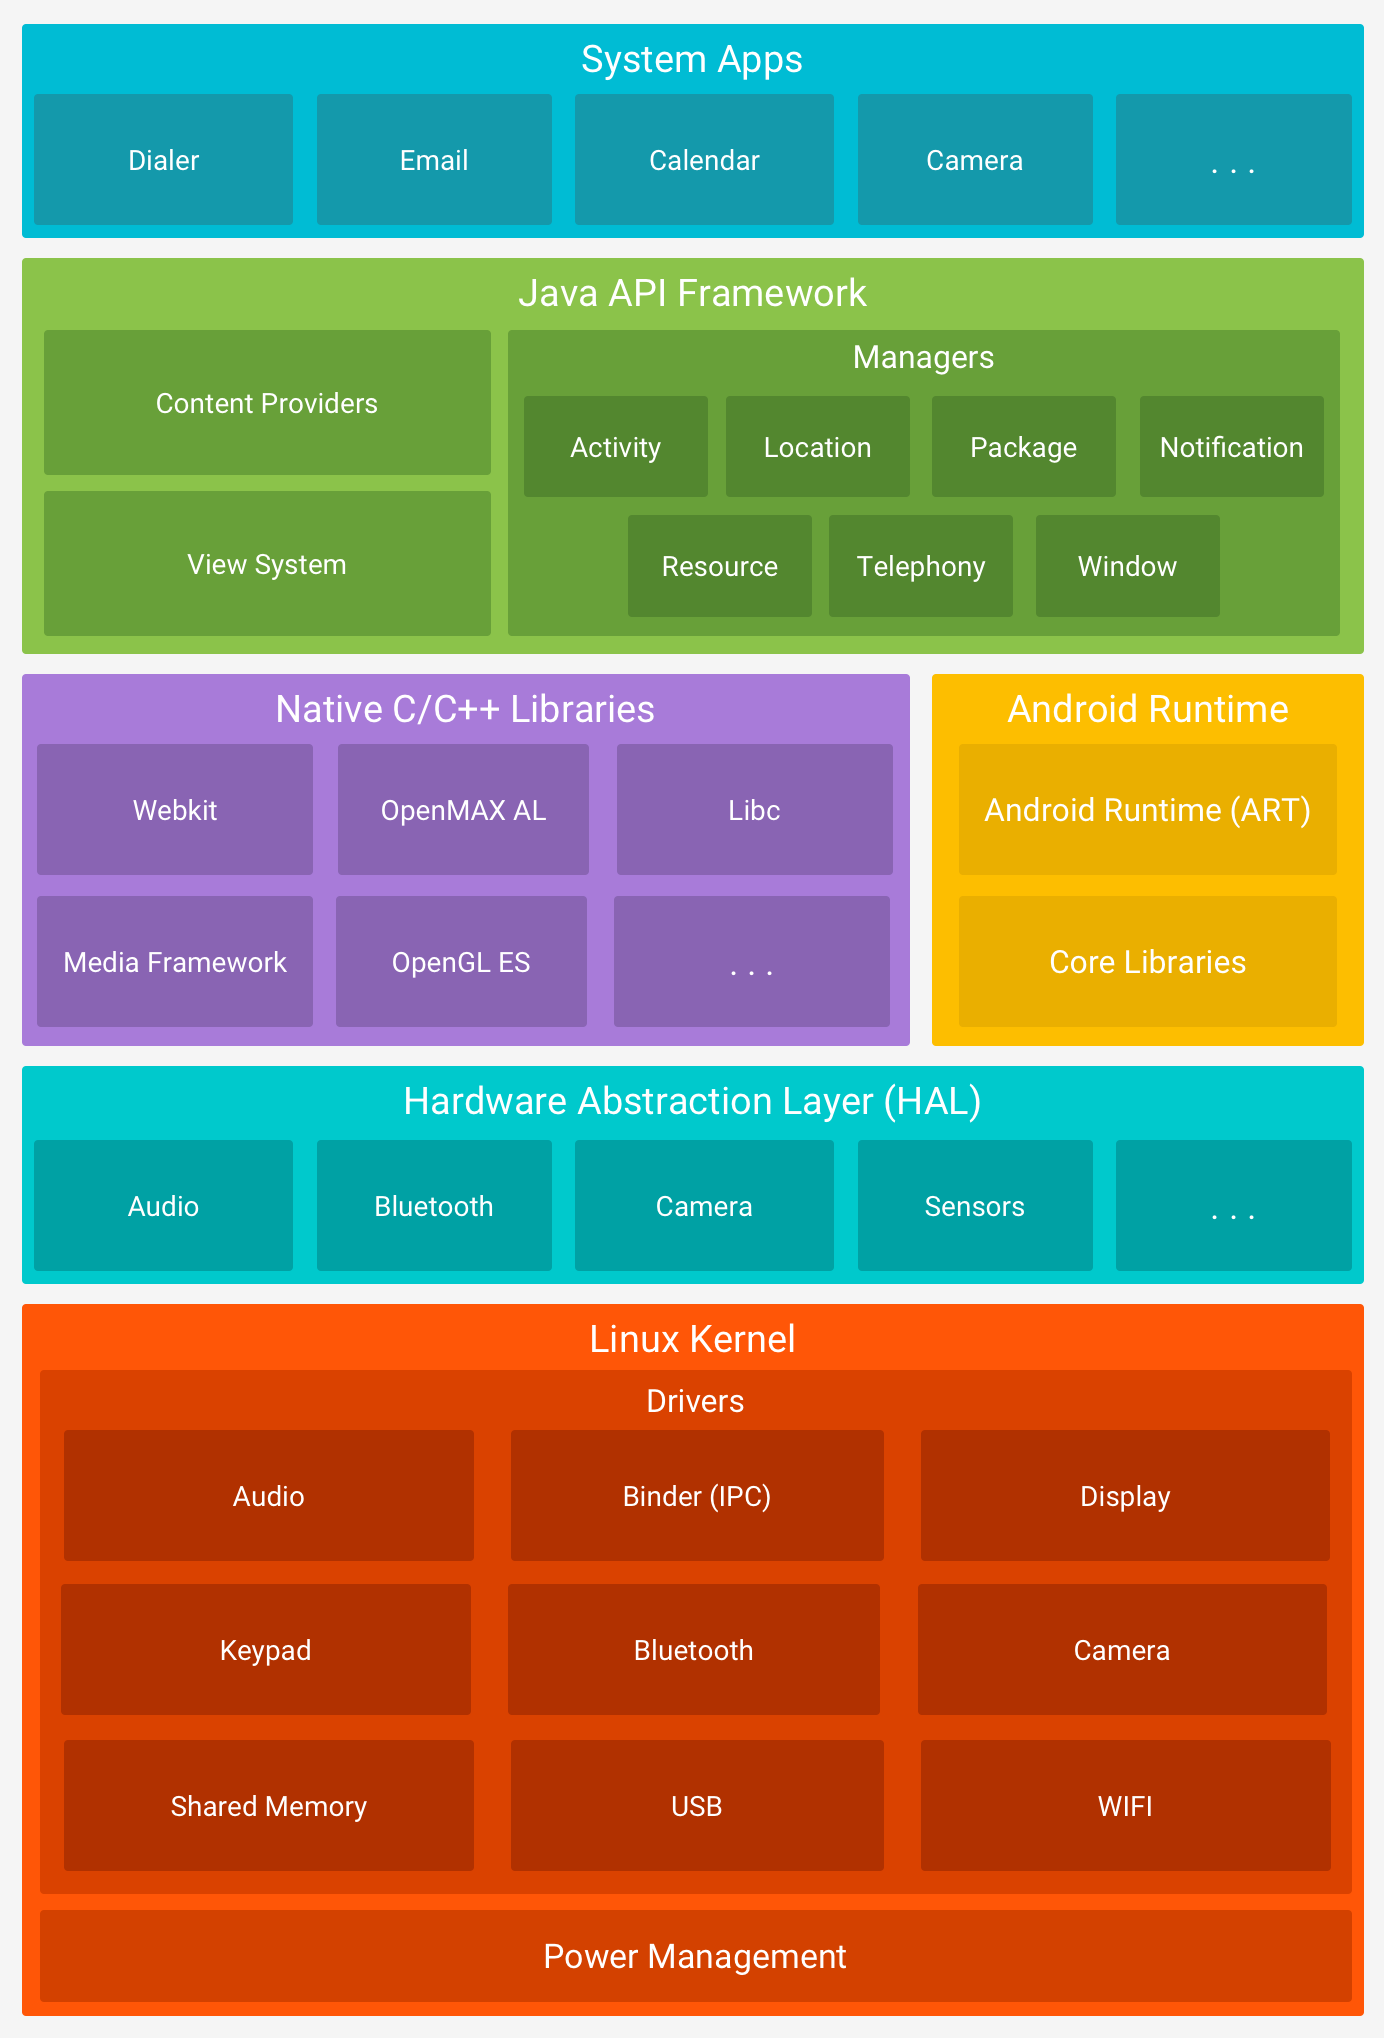
\includegraphics[scale=0.09]{../imagenes/android-stack.png}
            \end{figure}
        \end{column}
    \end{columns}
\end{frame}

\begin{frame}{Un poco de contexto sobre Android}{Componentes del sistema}
    \begin{itemize}[<+->]
        \item \textbf{Actividad}: representa una pantalla individual con interfaz de usuario
        \item \textbf{Servicio}: realiza operaciones de ejecución prolongada en segundo plano
        \item \textbf{Receptor de emisiones}: permite que el sistema u otras aplicaciones entreguen
              mensajes por fuera del flujo normal
        \item \textbf{Proveedor de contenido}: administra los datos de una aplicación para que
              puedan ser compartidos con otras
    \end{itemize}
\end{frame}

\begin{frame}{Un poco de contexto sobre Android}{Interacción entre componentes}
    \textit{Intents:} \\
    \begin{itemize}
        \item Mensajería utilizada para la comunicación entre componentes \pause
        \item Puden ser explícitos o implícitos
    \end{itemize}
    \vspace{20px} \pause
    Para recibir \textit{intents} implícitos, las aplicaciones declaran filtros de \textit{intents}.
    Este filtro se define en el \textbf{manifiesto} de la aplicación.
\end{frame}

\begin{frame}{Un poco de contexto sobre Android}{Permisos}
    Los recursos de una aplicación se protegen con distintos niveles de permisos.
    \begin{itemize}[<+->]
        \item Normal
        \item Peligrosos
        \item De misma firma
    \end{itemize}
    \vspace{20px} \pause Los permisos peligrosos se  otorgan en tiempo de ejecución. El resto, al
    instalar la aplicación.

    \vspace{20px} \pause Los permisos que pertenecen a una misma característica de una aplicación
    se agrupan en lo que definimos \textbf{grupo de permisos.}
\end{frame}

\begin{frame}{Un poco de contexto sobre Android}{Cambios de comportamiento recientes I}
    \textbf{Sistema de archivos}\\
    \vspace{10px}
    \begin{itemize}
        \item Los directorios de las aplicaciones tienen permisos restringidos
        \item Evita la fuga de metadatos
        \item Utilizar el mecanismo de \textit{intents} como la única forma segura de compartir
              archivos
    \end{itemize}
    \vspace{10px}
    \pause
    Cambio introducido en Android 7.
\end{frame}

\begin{frame}{Un poco de contexto sobre Android}{Cambios de comportamiento recientes II}
    \textbf{Cambios en permisos agrupados} \\
    \vspace{10px}
    Antes de Android 8, al otorgar un permiso peligroso, se otorgaban de manera incorrecta el resto
    de los permisos del grupo.\\
    \vspace{5px}
    A partir de esta versión de Android se corrige ese comportamiento y se define una noción de
    ``otorgamiento automático'' para permisos peligrosos.

    \vspace{10px} \pause
    \textbf{Permisos normales y peligrosos compartiendo grupo} \\
    \begin{block}{}
        ``Cualquier permiso puede pertenecer a un grupo de permisos sin importar el nivel del
        protección del mismo''
    \end{block}
    \pause
    ¿Cómo se comporta el sistema en este caso?
\end{frame}

\begin{frame}{Un poco de contexto sobre Android}{Cambios de comportamiento recientes III}
    \textbf{Chequeo de permisos en aplicaciones viejas} \\
    \vspace{10px}
    Alerta al usuario ante la ejecución de una aplicación cuyos permisos peligrosos fueron otorgados
    en tiempo de instalación.
\end{frame}

\begin{frame}{Nuestra formalización del sistema de permisos}{Consideraciones generales}
    Lenguaje formal utilizado: Coq
    \vspace{10px}
    \begin{block}{}
        Coq es un \textit{framework} que provee un lenguje formal para escribir definiciones
        matemáticas, algoritmos ejecutables y teoremas, junto con un entorno semi-interactivo para
        escribir demostraciones con la asistencia de una computadora.
    \end{block}
\end{frame}

\begin{frame}[fragile]
    \frametitle{Nuestra formalización del sistema de permisos}
    \framesubtitle{Definiciones básicas I}
    \textbf{Tipos atómicos}
    \begin{verbatim}
(* Certificado con el que se firma una aplicación *)
Parameter Cert: Set.
    \end{verbatim}
    \pause

    \textbf{Tipos inductivos}
    \begin{verbatim}
(* Tipos de Intents *)
Inductive intentType : Set :=
    | intActivity
    | intService
    | intBroadcast.
    \end{verbatim}
\end{frame}

\begin{frame}[fragile]
    \frametitle{Nuestra formalización del sistema de permisos}
    \framesubtitle{Definiciones básicas II}
    \textbf{Estructura de registros} (o tipos \textit{record})
    \begin{verbatim}
(* Manifiesto de una aplicación *)
Record Manifest : Set := mf {  cmp: list Cmp;
                            minSdk: option nat;
                            targetSdk: option nat;
                            use: list Perm;
                            usrP: list Perm; 
                            appE: option Perm }.
    \end{verbatim}
\end{frame}

\begin{frame}{Nuestra formalización del sistema de permisos}{Estado}
    \begin{columns}[T]
        \begin{column}{.45\textwidth}
            \textbf{Parte estática}
            \begin{itemize}
                \item Manifiestos
                \item Certificados
                \item Permisos definidos por aplicaciones
                \item Aplicaciones del sistema
            \end{itemize}
        \end{column}
        \pause
        \begin{column}{.55\textwidth}
            \textbf{Parte dinámica}
            \begin{itemize}
                \item Aplicaciones instaladas
                \item \textit{Apps legacy} verificadas
                \item Permisos otorgados
                \item Grupos de permisos validados
                \item Componentes en ejecución
                \item ...
            \end{itemize}
        \end{column}
    \end{columns}
\end{frame}

\begin{frame}{Nuestra formalización del sistema de permisos}{Acciones I}
    Acciones del modelo:
    \begin{itemize}[<+->]
        \item Representan operaciones reales de Android.
        \item En términos de nuestro modelo, son transiciones de estado.
        \item Su semántica está dada en términos de pre-condición y post-condición
    \end{itemize}
\end{frame}

\begin{frame}{Nuestra formalización del sistema de permisos}{Acciones II}
    \texttt{grant}\\
    \vspace{5px}
    Acción utilizada para otorgar permisos no agrupados o el primer permiso de un grupo en ser
    otorgado.\\
    \pause
    \vspace{10px}
    \texttt{grantAuto}\\
    \vspace{5px}
    Acción que simboliza el otorgamiento automático de permisos. La precondición se cumple solamente
    cuando el permiso está agrupado y cuando la aplicación ya cuenta con dicho grupo validado.
\end{frame}

\begin{frame}{Nuestra formalización del sistema de permisos}{Acciones III}
    \texttt{verifyOldApp}\\
    \vspace{5px}
    Modela el cambio introducido en Android 10 para re-chequear los permisos de las aplicaciones
    \textit{legacy}.
    \pause
    \vspace{10px}
    \texttt{receiveIntent}\\
    \vspace{5px}
    A partir de ahora, las aplicaciones \textit{legacy} podrán postularse para resolver
    \textit{intents} implícitos pero no podrán recibirlos si no fueron verificadas.
\end{frame}

\begin{frame}{Nuestra formalización del sistema de permisos}{Acciones IV}
    \texttt{revoke} y \texttt{revokePermGroup}\\
    \vspace{5px}
    Estas acciones se modificaron para mantenerse alineadas con la experiencia de usuario:
    \texttt{revoke} revoca permisos no agrupados y \texttt{revokePermGroup} elimina todos los
    permisos pertenecientes a ese grupo.\\
\end{frame}


\begin{frame}{Nuestra formalización del sistema de permisos}{Ejecuciones}
    Definimos una noción de ejecución a partir de una sucesión de acciones.

    \begin{displaymath}
        \fontsize{8pt}{9pt}\selectfont
        \begin{array}{c}
            \inference[]{$$valid\_state(s)$$ \hspace{.2cm} $$Pre(s, a)$$ \hspace{.2cm} $$Post(s, a, s')$$}{$$s\step{a/ok}s'$$}
            \hspace{0.5cm}
            \inference[]{$$valid\_state(s)$$ \hspace{.2cm} $$ErrorMsg(s, a, ec)$$}{$$s\step{a/error(ec)}s$$}
        \end{array}
    \end{displaymath}
    \pause
    \begin{theorem}{Las ejecuciones preservan la validez del estado}
        \fontsize{9pt}{12pt}\selectfont
        $\begin{array}{l} \forall\ (s\ s':\AndroidState)(a:\Action) (r:Response), s\step{a/r}s'
                \rightarrow valid\_state(s')\end{array}$
    \end{theorem}
\end{frame}

\begin{frame}{Trabajos relacionados}
    Divididos en tres categorías:
    \pause
    \begin{itemize}[<+->]
        \item De análisis informal:
              \begin{itemize}
                  \item Características nuevas, resumen de vulnerabilidades, mitigaciones
                  \item Complemento a la documentación oficial
              \end{itemize}
        \item Herramientas de análisis estático o dinámico:
              \begin{itemize}
                  \item Sobreprivilegios, flujo indebido de la información
                  \item Estudia casos de uso específicos
              \end{itemize}
        \item De análisis formal:
              \begin{itemize}
                  \item Estudiar escenarios específicos mediante algún lenguaje formal
                  \item Especificaciones de la plataforma (en lenguajes como TLA+, Alloy, Coq)
              \end{itemize}
    \end{itemize}
\end{frame}

\begin{frame}{Conclusiones}
    \begin{itemize}[<+->]
        \item Actualizamos la formalización a una versión reciente de la plataforma
        \item Analizamos la validez de las propiedades existentes y generamos nuevas, en particular,
              relacionadas a los cambios de comportamiento de los grupos de permisos
        \item Como consecuencia de la actualización en la formalización, actualizamos la
              implementación informal  y su prueba de corrección.
    \end{itemize}
\end{frame}

\begin{frame}{Trabajo futuro}
    \begin{itemize}[<+->]
        \item Utilizar el código extraído para comparar y validar ejecuciones reales de la
              plataforma
        \item Utilizar el código extraído para generar casos de prueba
        \item Continuar actualizando la especificación con los cambios introducidos en Android 11 y
              12.
              \begin{itemize}
                  \item Reestablecimiento de permisos en aplicaciones inactivas
                  \item Permisos de un único uso
              \end{itemize}
    \end{itemize}
\end{frame}

\begin{frame}{Fin}
    \begin{center}
        \huge¡Gracias!
    \end{center}
\end{frame}

% Extra slides just in case
\begin{frame}{Definición formal del estado}{Parte dinámica}
    \fontsize{10pt}{11pt}\selectfont
    \begin{flalign*}
        State\ &:=\ \{ &&\\
        &apps:\ list\ idApp; \\
        &alreadyVerified:\ list\ idApp; \\
        &grantedPermGroups:\ mapping\ idApp\ (list\ idGrp); \\
        &perms:\ mapping\ idApp\ (list\ Perm); \\
        &running:\ mapping\ iCmp\ Cmp; \\
        &delPPerms:\ mapping\ (idApp\ *\ CProvider\ *\ uri)\ PType; \\
        &delTPerms:\ mapping\ (iCmp\ *\ CProvider\ *\ uri)\ PType; \\
        &resCont:\ mapping\ (idApp\ *\ res)\ Val; \\
        &sentIntents:\ list\ (iCmp*Intent) \\
        \}
    \end{flalign*}
\end{frame}

\begin{frame}{Definición formal del estado}{Parte estática}
    \fontsize{10pt}{11pt}\selectfont
    \begin{flalign*}
        Environment\ &:=\ \{ &&\\
        &manifest:\ mapping\ idApp\ Manifest; \\
        &cert:\ mapping\ idApp\ Cert; \\
        &defPerms:\ mapping\ idApp\ (list\ Perm); \\
        &systemImage:\ list\ SysImgApp; \\
        \}
    \end{flalign*}
    \begin{align*}
        System\ :=\ \{ state: State;\ environment: Environment \}
    \end{align*}
\end{frame}
\end{document}